\documentclass{report}
\usepackage{graphicx} % Required for inserting images
\usepackage[italian]{babel} %use this package for a thesis written in Italian
\usepackage[utf8]{inputenx}
\usepackage{indentfirst}
\usepackage{microtype}
%\usepackage{chemformula}
\usepackage{mhchem}
\usepackage{setspace}
\usepackage{yfonts,color}
%\usepackage{siunitx}
\usepackage{comment}
%\usepackage{multirow}
%\usepackage{varioref}
%\usepackage[bottom]{footmisc}
\usepackage{wrapfig}
%\usepackage{float}
%\usepackage{type1cm}
\usepackage{lettrine}
\linespread{1.1}
%\usepackage{chngcntr}
\usepackage[nottoc, notlof, notlot]{tocbibind}
%\onehalfspacing
%\counterwithout{footnote}{chapter}
\usepackage{hyperref}
\usepackage[margin=3cm]{geometry}
\usepackage{titlesec}
\titleformat{\section}
  {\color{teal}\normalfont\Large\bfseries}
  {\thesection}{1em}{}
\titleformat{\subsection}
  {\color{teal!80}\bfseries\normalfont\large}
  {\thesubsection}{1em}{}

\usepackage{caption}
\usepackage{subcaption}

\usepackage{booktabs}
\usepackage{tabularx}
\usepackage{adjustbox}
\usepackage{multirow}
\usepackage{multicol}
\usepackage{listings}
\usepackage{matlab-prettifier}

\usepackage{lipsum}

\lstset{
    language=Matlab,
    style= Matlab-editor,
    basicstyle=\ttfamily\small,
    numbers=left,
    numberstyle=\tiny,
    stepnumber=1,
    numbersep=8pt,
    breaklines=true,
    frame=single,
    showstringspaces=false,
    tabsize=4
}

\hypersetup{
			hyperfootnotes=true,			
			bookmarks=true,			
			colorlinks=true,
			linkcolor=blue,
            linktoc=page,
			anchorcolor=black,
			citecolor=blue,
			urlcolor=blue,
			pdftitle={Tesi Risi},
			pdfauthor={Lorenzo Risi},
			pdfkeywords={thesis, sapienza, roma, university}
 }


\title{Modelli di sistemi biologici\\Modulo Pietro Aricò}
\author{Lorenzo Risi}
\date{September 2026}

\begin{document}
\maketitle
\tableofcontents

\chapter{Richiami di elettrofisiologia cellulare e
registrazioni su singola cellula}
Al termine di questo capitolo potremmo:
\begin{itemize}
    \item Elencare le 3 principali funzioni della cellula neuronale
    \item Descrivere la struttura specializzata che permette al neurone di svolgere le sue funzioni
    \item Scrivere l’equazione di Nernst, spiegarne il significato e usarla per determinare la direzione di spostamento di una famiglia ionica
    \item Descrivere i principali meccanismi di trasporto di membrana e
riconoscere se si tratta di trasporto passivo o attivo
    \item Descrivere il funzionamento della pompa sodio-potassio
    \item Indicare qual è il potenziale di riposo della membrana neuronale e
descrivere i tre fenomeni concomitanti che lo determinano
    \item Comprendere l’effetto depolarizzante o iperpolarizzante/ripolarizzante di ciascuna famiglia ionica sulla membrana neuronale
\end{itemize}

\section{Struttura del neurone, potenziale di membrana, meccanismi di trasporto} La struttura del neurone è legata alle sue 3 funzioni:
\begin{itemize}
    \item \textbf{Ricezione} di informazioni da più
sorgenti (altre cellule nervose,
recettori, segnali inibitori o
eccitatori)
    \item \textbf{Integrazione} (nel tempo e nello spazio) dell’informazione raccolta per fornire una risposta binaria (se la somma supera una certa soglia)
    \item \textbf{Generazione e propagazione} di un bit di informazione verso altre cellule (nervose, muscolari), il potenziale d’azione
\end{itemize}
In sintesi, il neurone funziona come un elaboratore biologico di informazioni: riceve, elabora e trasmette segnali in modo molto rapido ed efficiente
\begin{figure}
    \centering
    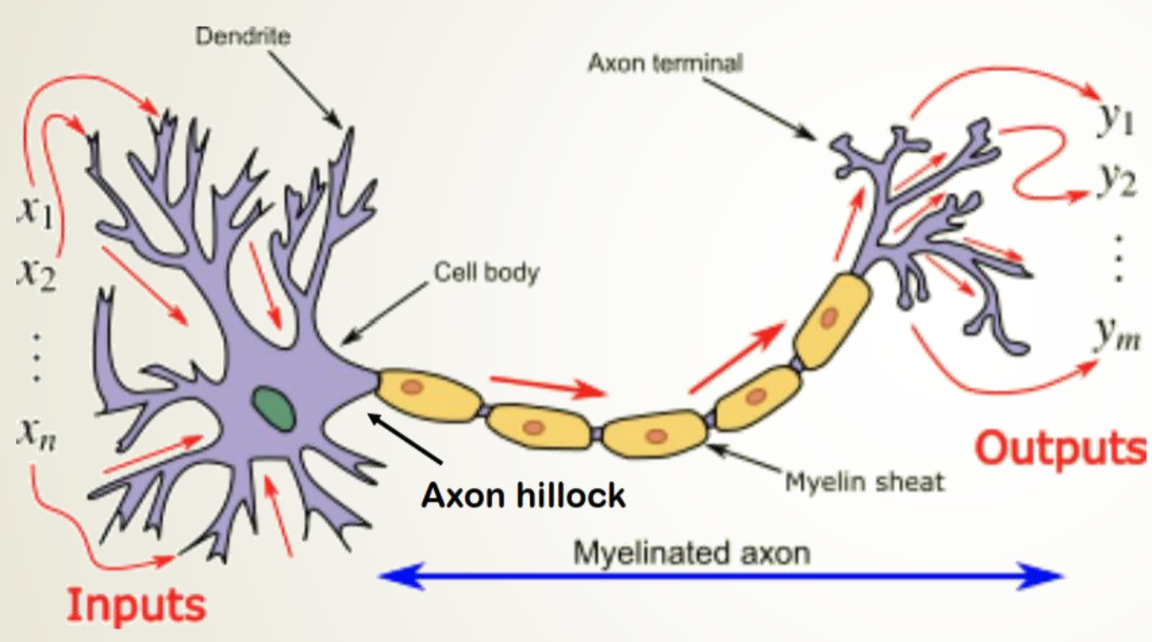
\includegraphics[width=0.7\linewidth]{immagini/neurone.png}
    \caption{Sistema di input della cellula nervosa}
    \label{fig:placeholder}
\end{figure}
I dendriti sono dei recettori che prendono in ingresso un potenziale ($x_1,x_2,x_3$), nel cono di emergenza (axon hillock) viene filtrato il segnale: se è abbastanza forte il segnale passa all'assone. In questo caso abbiamo delle guaine mieliniche che permettono di velocizzare la trasmissione del potenziali di azione sui vari nodi. Infine il potenziale arriva sui terminali assonici ($y_1,y_2,y_3$) i quali sono connessi, per via delle sinapsi, ai dendriti del neurone post-sinaptico per propagare l'informazione. 

\medskip
La struttura della membrana neuronale è composta da un doppio strato fosfolipidico dove 1 fosfolipide è formato da una testa fosforica e 2 code di acidi grassi: \textbf{Teste polari} (idrofile) sul versante extracellulare e citoplasmatico (ambienti idrofili), \textbf{Code idrofobe} (lipofile) all’interno della membrana (barriera al passaggio incontrollato di sostanze idrosolubili). Per avere uno scambio tra interno ed esterno abbiamo le proteine globulari di membrana:
\begin{itemize}
    \item \textbf{Proteine integrali}: attraversano tutto lo spessore di membrana sporgendo sia all’interno che all’esterno della cellula. Possono formare canali o trasportatori per il passaggio di ioni e molecole.

    \item \textbf{Proteine periferiche}: sono sul versante esterno (es recettori) o interno (es. enzimi). Legate alla membrana ma possono essere rimosse
\end{itemize}
Le principali famiglie ioniche coinvolte sono: sodio, potassio, cloruro, calcio ($\ce{Na+,K+,Cl-,Ca++}$). Abbiamo una diversa concentrazione di ioni ai due versanti della membrana cellulare, il mantenimento della differenza elettrochimica ai due lati della membrana è reso possibile dalla sua permeabilità selettiva agli ioni, il passaggio viene controllato grazie ai canali ionici. La differenza di potenziale elettrico tra l'interno di un neurone e il fluido extracellulare che lo circonda genera il \textbf{potenziale di membrana} \ref{fig:Potenziale di membrana}. Questa ddp è causata dalla differenze concentrazione di ioni ai due lati della membrana.
\begin{figure}
    \centering
    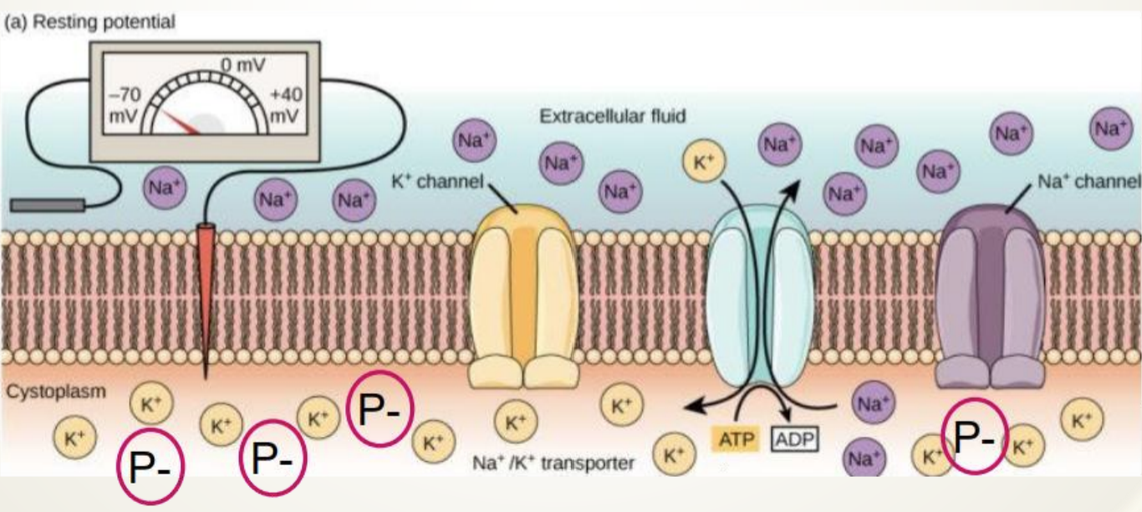
\includegraphics[width=0.75\linewidth]{immagini/potenzialedimembrana.png}
    \caption{Potenziale di membrana}
    \label{fig:Potenziale di membrana}
\end{figure}
L'equilibrio elettrochimico dipende dall'equilibrio delle due forze in gioco: 
\begin{itemize}
    \item Forze di diffusione: sono dovute al gradiente chimico
(differenza di concentrazione degli ioni di una
famiglia nel fluido intra- ed extra-cellulare)
    \item Forze elettriche: gli ioni positivi sono attratti verso la
regione con un potenziale negativo, e viceversa
(gradiente elettrico)
\end{itemize}
L’effetto sommato di queste forze, quindi il punto in
cui si bilanciano, dà origine ad un equilibro
elettrochimico, dato dall’equazione di Nernst:
\begin{equation}
    \Delta\mu= \colorbox{red!40}{$\displaystyle RT\frac{[X]_A} {[X]_B}$} + \colorbox{blue!50}{$zF(E_A-E_B)$}
\end{equation}
Questa espressione descrive l’energia necessaria (o disponibile)
per il trasporto di uno ione X da un compartimento B a un
compartimento A, tenendo conto sia del gradiente di
concentrazione che della differenza di potenziale elettrico. La parte rossa rappresenta l'energia termica delle molecole che induce un movimento causale delle stesse: questo tende a spostare gli ioni secondo gradiente di concentrazione, Se $[X]A > [X]B$, lo ione tende ad andare da A verso B, e viceversa. In blu abbiamo l'energia potenziale persa o guadagnata attraversando una differenza di potenziale pari a $(E_A -E_B)$, e dipendente dalla carica. Tende a spostare gli ioni secondo gradiente
elettrico, se lo ione è positivo ($z>0$), sarà attratto verso il
compartimento più negativo, e viceversa.

\bigskip
Finché  $\Delta\mu\ne0$ ci sarà uno spostamento netto di ioni dovuto al gradiente elettrochimico. Ponendo $\Delta\mu =0$ (equilibrio elettrochimico) e considerando ambiente extra
(E) ed intracellulare (I), abbiamo:
\begin{equation}
\begin{split}
     &RT \ln \frac{[X]_E}{[X]_I} + zF(E_E - E_I) = 0 \rightarrow -zF(E_E - E_I) = RT \ln \frac{[X]_E}{[X]_I}
    \\
    &E_I - E_E = E_j = \frac{RT}{Fz} \ln \left( \frac{[extra]_i}{[intra]_j} \right)
\end{split}
\end{equation}
$E_j$ è il potenziale in cui le forze di diffusione secondo gradiente di
concentrazione bilanciano quelle secondo gradiente elettrico per gli ioni
di tipo j. Valori tipici del potenziale di equilibrio elettrochimico:
\begin{itemize}
    \item Potassio: EK+ = -90mV
\item Sodio: ENa+ = 50 mV
\item Calcio: ECa++ = 150 mV
\item Cloro: ECl- = -65 mV
\end{itemize}
Un potenziale di equilibrio Ej tende a spostare il potenziale di membrana
(che di solito è circa -70mV a riposo) verso quel valore, gli ioni si
sposteranno verso l’interno o verso l’esterno a seconda del loro segno.

\subsection{Meccanismi di trasporto}
Gli ioni si possono muovere in due modi: 
\begin{itemize}
    \item \textbf{Trasporto passivo} per gradiente elettrochimico.
Usa l’energia degli ioni e non richiede uso di ATP
(Adenosina Trifosfato) da parte della cellula. Ad esempio: i meccanismi di trasporto passivo fanno spostare
$\ce{Na+}$ verso l’interno e $\ce{K+}$ verso l’esterno (coerentemente
con Nernst)

\item \textbf{Trasporto attivo} (pompe ioniche). Richiede l'impiego di energia per spostare gli ioni contro gradiente. Ad esempio la pompa sodio-potassio (crea il potenziale di
membrana): butta fuori 3 Na+, fa entrare 2 K+ e usa 1 molecola di ATP ogni ciclo
\end{itemize}

Le pompe ioniche spostano gli ioni \emph{contro il loro gradiente} elettrochimico mediante trasporto attivo. La più importante è la pompa sodio-potassio fondamentale per mantenere il potenziale di membrana al
suo valore nominale ($-70$ mV per i neuroni). Quando la membrana è a riposo (potenziale di $-70$ mV) si dice che la membrana è polarizzata. Se una corrente di ioni positivi entra nella cellula e il potenziale di membrana diventa positivo superando una determinata soglia la membrana di \textbf{depolarizza}. Quando una corrente di ioni positivi esce dalla cellula il potenziale di membrana torna negativo e si ripolarizza, nel caso in cui superi i $-70$ mV si parla di iperpolarizzazione (massimo $-80$ mV).
\begin{figure}[h!]
    \centering
    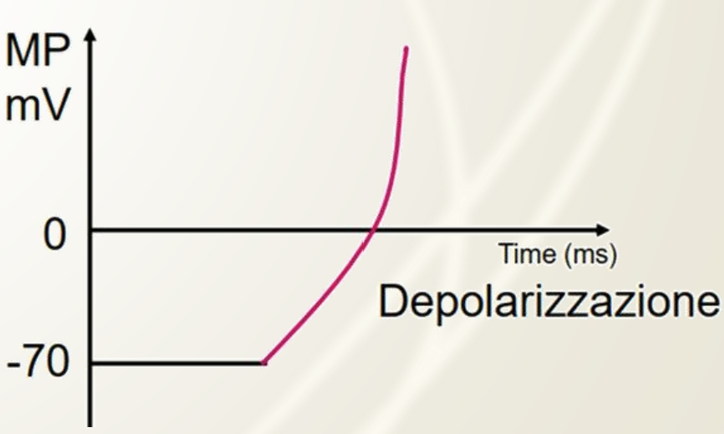
\includegraphics[width=0.4\linewidth]{immagini/depolarizzazione.png}
    \quad
    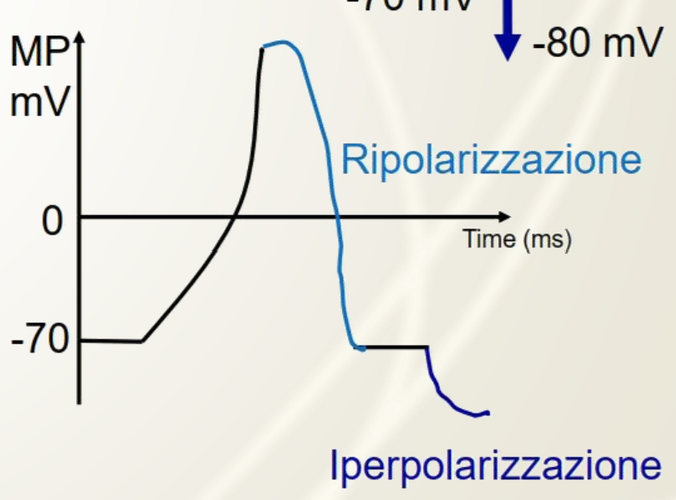
\includegraphics[width=0.35\linewidth]{immagini/ripolarizzazione.png}
    \caption{Enter Caption}
    \label{fig:placeholder}
\end{figure}

\noindent La diffusione facilitata avviene attraverso i canali ionici, alcune proteina canale hanno proprietà selettive per certi ioni. Alcuni canali sono sempre aperti, altri si aprono e chiudono in risposta a eventi chimici, elettrici o meccanici: \textbf{canali a cancello}. 

\subsubsection{Il canale $\ce{Na+}$ voltaggio-dipendente}
Al potenziale di riposo questo canale è chiuso, quando il potenziale arriva a $-60$ mV si apre e gli ioni possono attraversarlo. La soglia di inattivazione è a $+30$ mV, gli ioni non possono attraversarlo e non può essere attivato. Quando si ritorna alla soglia di chiusura, potenziale di riposo, rimane chiuso ma può essere attivato.
\subsubsection{Il canale $\ce{K+}$ voltaggio-dipendente}
Al potenziale di riposo questo canale è chiuso, quando il potenziale arriva a $+30$ mV si apre e gli ioni possono attraversarlo. La soglia di inattivazione è a $-80$ mV, gli ioni non possono attraversarlo e non può essere attivato. Quando si ritorna alla soglia di chiusura, potenziale di riposo, rimane chiuso ma può essere attivato.

\begin{table}[h!]
\centering
\renewcommand{\arraystretch}{1.5}
\begin{tabular}{|c|cccc|}
\hline
\textbf{Canale} & \textbf{Potenziale} & \textbf{Stato del canale} & \textbf{Cosa fanno gli ioni} & \textbf{Effetto sulla membrana} \\
\hline
Na$^+$, K$^+$ & -70 mV & Chiuso (riposo) & Nessun passaggio & Pronto ad aprirsi \\
\hline
Na$^+$ & -60 mV & Aperto (attivato) & Na$^+$ entra nella cellula & Depolarizzazione \\
\hline
Na$^+$ & +30 mV & Inattivo & Nessun passaggio & Fine ingresso Na$^+$ \\
\hline
K$^+$ & +30 mV & Aperto (attivato) & K$^+$ esce dalla cellula & Ripolarizzazione \\
\hline
K$^+$ & -80 mV & Chiuso (chiusura ritardata) & Nessun passaggio & Iperpolarizzazione \\
\hline
Na$^+$, K$^+$ & -70 mV & Chiuso (riposo) & Nessun passaggio & Pronto ad aprirsi \\
\hline
\end{tabular}
\end{table}
\section{Generazione e propagazione del potenziale d'azione, potenziali graduati} 
Il potenziale d'azione è una variazione del potenziale che si propaga lungo la membrana, questo è caratteristico delle cellule eccitabili. Il principio di funzionamento è "tutto o nulla": se lo stimolo non raggiunge una certa soglia di depolarizzazione non avviene, al contrario, se la soglia è raggiunta, il PA si ripete sempre con lo stesso andamento, intensità e durata. Il processo di divide in 4 fasi: 
\begin{itemize}
    \item \textbf{Fase 1} depolarizzazione fino al valore di soglia
    \item \textbf{Fase 2} attivazione dei canali $\ce{Na+}$ e rapida depolarizzazione
    \item \textbf{Fase 3}: Inattivazione dei
canali del Na+ e attivazione
dei canali del K+
    \item \textbf{Fase 4}: Ripolarizzazione dovuta alle correnti
ripolarizzanti di K+ (K+ esce dalla cellula). Undershoot (iperpolarizzazione) finché in canali K+ non si richiudono (-80) Ritorno al potenziale di riposo dovuto alla pompa sodio-
potassio e ai canali di perdita
\end{itemize}
La \textbf{refrattarietà assoluta} è l'intervallo di tempo in cui i canali del $\ce{Na+}$ sono inattivi e non possono riaprirsi. Durante questo intervallo è impossibile che si generi un nuovo potenziale d'azione, per quanto forte sia lo stimolo. Termina quando il potenziale di membrana torna ai $-70$ mV).\\
La \textbf{refrattarietà relativa} è l'intervallo di tempo in cui il potenziale di membrana scende sotto il valore di riposo a causa dell’apertura dei canali del $\ce{K+}$. Durante questo intervallo è meno probabile, ma non impossibile che si generi un nuovo potenziale d’azione. Serve uno stimolo più forte.
Termina quando i canali $\ce{K+}$ si chiudono ($-80$ mV).
\medskip
\begin{figure}[h!]
    \centering
    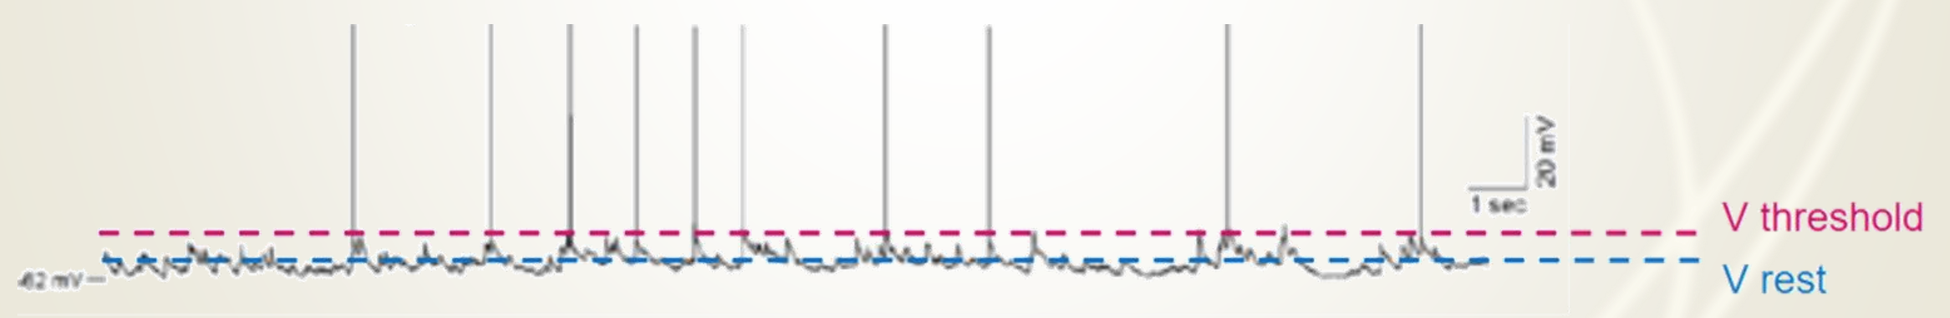
\includegraphics[width=1\linewidth]{immagini/potenziale dazione.png}
    \caption{potenziali d'azione}
    \label{fig:placeholder}
\end{figure}
\newpage
\subsection{Propagazione del potenziale d'azione}
Una volta generato il potenziale di azione in un particolare punto della membrana (in genere in corrispondenza del cono di
emergenza dell’assone) questo si propaga lungo la struttura
dell’assone: assoni più grandi, resistenza al flusso
minore. Ci sono 2 principali tipi di propagazione: continua (fibre amieliniche) e saltatoria (fibre mielinizzate) .
\subsubsection{Propagazione continua}
\noindent La rapida depolarizzazione di membrana provoca correnti ioniche
intra- ed extracellulari (secondo gradiente elettrochimico) che
propagano la perturbazione a tutte le porzioni adiacenti di membrana (in ogni direzione). La perturbazione depolarizzante
innesca nuovamente il potenziale d’azione (rigenerazione attiva) dove incontra canali Na+ pronti ad aprirsi. 
\begin{figure}[h!]
    \centering
    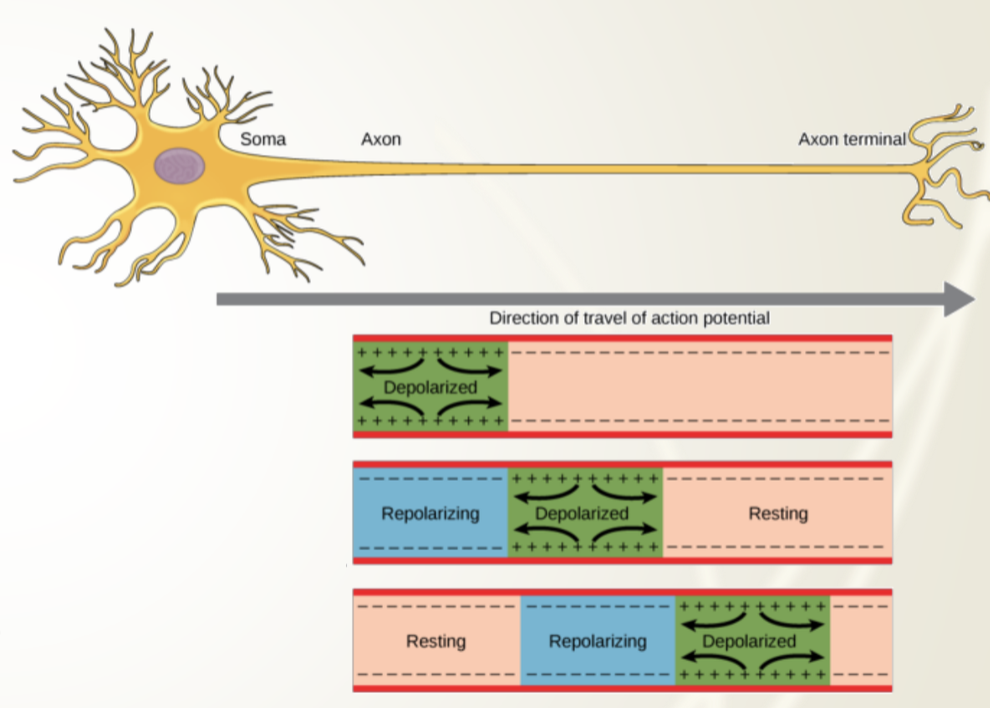
\includegraphics[width=0.75\linewidth]{immagini/porpagazionecontinua.png}
    \caption{Propagazione continua}
    \label{fig:placeholder}
\end{figure}
Se la porzione adiacente di membrana ha appena generato a sua volta un potenziale d'azione, si troverà nel periodo di refrattarietà assoluta quindi sarà impossibile generare un nuovo
potenziale d'azione. La velocità di propagazione è di $1$ m/s ed è limitata dai processi di attivazione dei canali $\ce{Na+\,e\,K+}$.
\subsubsection{Propagazione saltatoria}
La presenza di un isolante (guaina mielinica),
costituito da cellule di Schwann oppure
oligodendrociti, avvolti a spirale su sé stessi e
intervallati da punti in cui la membrana è
scoperta (nodi di Ranvier) porta all'alternarsi di propagazione passiva (lungo la sezione mielinizzata) e rigenerazione attiva del potenziale (in corrispondenza dei nodi): il potenziale «salta» da un nodo all'altro. In questo modo si ha una minore dispersione del segnale e la velocità di propagazione arriva fino a $120$ m/s. Le vie motorie sono mielinizzate mentre quelle dolorifiche no. 




\section{La trasmissione sinaptica e l'integrazione
dell'informazione da parte della cellula nervosa}

I neuroni sono cellule specializzate nella raccolta, nell'elaborazione e nella trasmissione di informazioni. \textbf{L'albero dendritico} di un neurone (composto da dendriti apicali e basali) rappresenta la principale stazione di ricezione dei segnali provenienti da altri neuroni o recettori sensoriali, comunicando attraverso giunzioni specializzate chiamate \textbf{sinapsi}. Una singola cellula nervosa può ricevere da 1 a 100.000 ingressi sinaptici. Poiché i segnali in entrata sono molteplici, il neurone postsinaptico funge da \textbf{integratore}, sommando gli effetti di questi stimoli sia nel tempo che nello spazio.

\subsection{Tipologie di Sinapsi}

La \textit{trasmissione delle informazioni} tra neuroni può avvenire attraverso due meccanismi principali: la sinapsi elettrica e la sinapsi chimica.

\subsubsection{Sinapsi Elettriche}
Nelle sinapsi elettriche, la trasmissione del segnale avviene in \textit{modo diretto} grazie a una continuità citoplasmatica tra le due cellule comunicanti. Questa continuità è garantita dalle \textbf{giunzioni comunicanti} (gap junctions), formate da complessi proteici chiamati connessoni (a loro volta costituiti da connessine), che riducono lo spazio intercellulare a circa 3,5 nm. 

I principali vantaggi di questo tipo di sinapsi sono l'elevata velocità di trasmissione (particolarmente utile nei riflessi rapidi) e la capacità di sincronizzare l'attività di interi gruppi cellulari, come avviene nel muscolo cardiaco o nella retina.
\begin{figure}[h!]
    \centering
    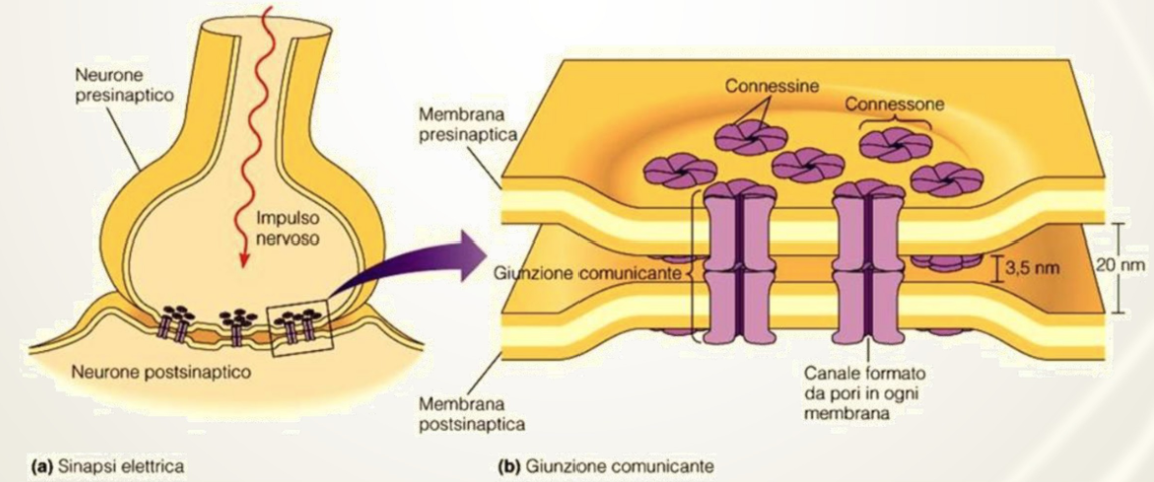
\includegraphics[width=0.8\linewidth]{immagini/sinapsielettrica.png}
\end{figure}
\subsubsection{Sinapsi Chimiche}
A differenza di quelle elettriche, le sinapsi chimiche presentano uno spazio fisico che separa le due cellule, denominato fessura sinaptica (circa 20 nm). In questo caso, lo scambio di informazioni è strettamente unidirezionale: dal neurone presinaptico (che trasmette l'informazione) al neurone postsinaptico (che la riceve). Il segnale elettrico originale deve essere \textbf{convertito} in un segnale chimico per attraversare la fessura, per poi essere riconvertito in segnale elettrico.
\newpage
Il processo si articola in diverse fasi sequenziali:
\begin{enumerate}
    \item Il potenziale d'azione invade il bottone presinaptico.
    \item La depolarizzazione provoca l'apertura dei canali per il \textbf{Calcio} ($\mathrm{Ca}^{2+}$) voltaggio-dipendenti, che si attivano a una soglia di circa +40 mV.
    \item Gli ioni $\mathrm{Ca}^{2+}$ fluiscono all'interno della cellula presinaptica spinti dal proprio gradiente elettrochimico.
    \item L'ingresso del calcio induce l'\textit{esocitosi delle vescicole sinaptiche}, liberando i neurotrasmettitori nella fessura sinaptica.
    \item Le molecole di neurotrasmettitore si legano a specifici recettori posti sulla membrana postsinaptica.
    \item Il legame determina l'apertura dei canali ionici postsinaptici, causando una depolarizzazione o iperpolarizzazione della membrana.
    \item Il segnale si interrompe quando il neurotrasmettitore viene allontanato dalla fessura sinaptica (tramite degradazione enzimatica, riassorbimento cellulare o semplice diffusione), permettendo la chiusura dei canali.
\end{enumerate}
\begin{figure}[h]
    \centering
    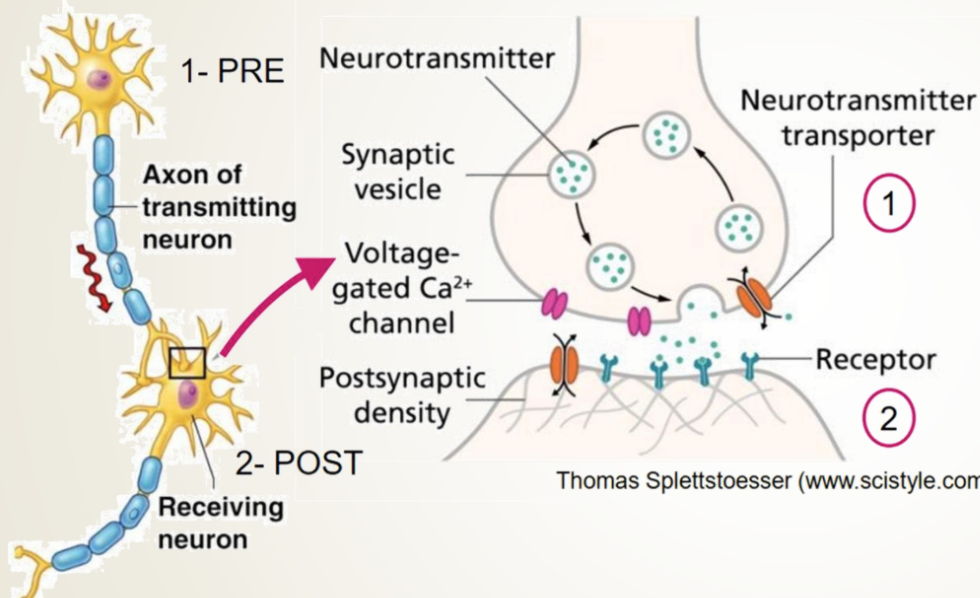
\includegraphics[width=0.65\linewidth]{immagini/sinapsichimica.png}
    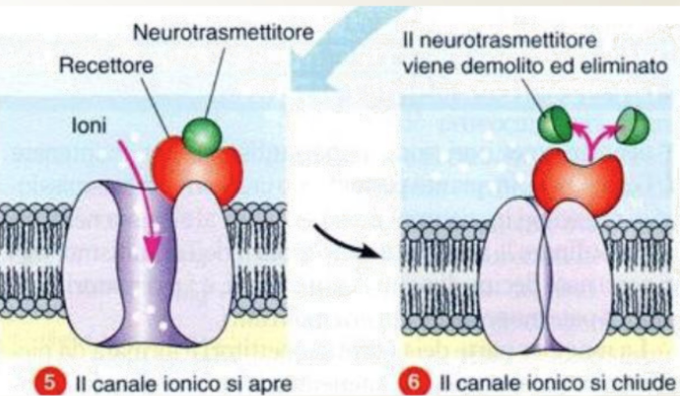
\includegraphics[width=0.65\linewidth]{immagini/neurotrasmettitore.png}
\end{figure}

\subsection{Classi di Recettori Sinaptici}
\iffalse
\begin{wrapfigure}{r}{0.3\textwidth}
  \centering
  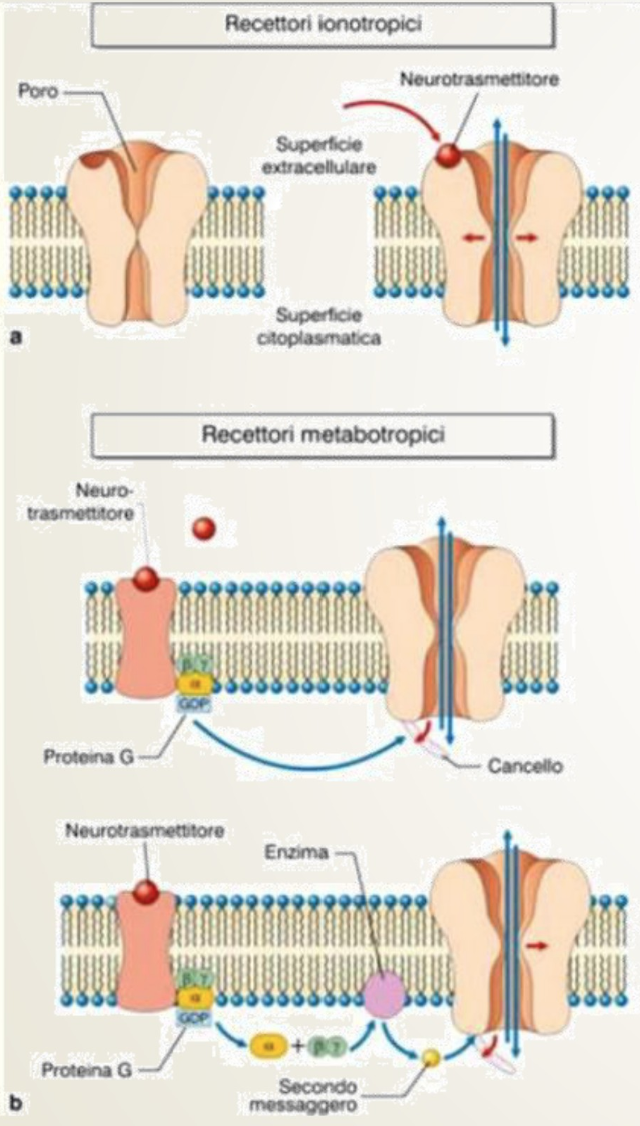
\includegraphics[width=0.3\textwidth]{immagini/ionotropicometabotropico.png}
\end{wrapfigure}
\fi
I recettori postsinaptici si dividono in due grandi categorie a seconda del loro meccanismo di azione:
\begin{itemize}
    \item \textbf{Recettori Ionotropici:} Il neurotrasmettitore si lega direttamente al canale ionico, causandone l'immediata apertura. Si tratta di un meccanismo di attivazione e disattivazione molto rapido, tipico dei circuiti che governano i riflessi motori.
    \item \textbf{Recettori Metabotropici:} Il neurotrasmettitore si lega a un recettore separato dal canale ionico. Questo legame attiva una Proteina G che avvia la produzione di ``secondi messaggeri'' intracellulari. Saranno questi ultimi ad agire dall'interno per aprire i canali ionici. È un processo più lento, ma in grado di indurre \textit{cambiamenti metabolici a lungo termine} legati ai fenomeni di plasticità sinaptica, apprendimento e memoria.
\end{itemize}

\subsection{Integrazione dell'Informazione e Potenziali}

L'attività sinaptica produce variazioni del potenziale di membrana locale note come potenziali postsinaptici (PSP), che hanno un'ampiezza di circa 1 mV e una durata di 15 ms. L'azione eccitatoria o inibitoria avviene sul singolo dendrite e viene poi integrata con le altre informazioni.

Se la sinapsi è \textbf{eccitatoria} (ad esempio mediata dal glutammato, che causa l'ingresso di $\mathrm{Na}^{+}$), si registra una depolarizzazione definita Potenziale Postsinaptico Eccitatorio (EPSP). 

Se la sinapsi è \textbf{inibitoria} (ad esempio mediata dal GABA, che causa l'uscita di $\mathrm{K}^{+}$), si verifica un'iperpolarizzazione nota come Potenziale Postsinaptico Inibitorio (IPSP). I termini ``eccitatorio'' e ``inibitorio'' sono sempre riferiti alla probabilità di raggiungere la soglia per l'innesco di un potenziale d'azione.


\begin{figure}[h]
    \centering
    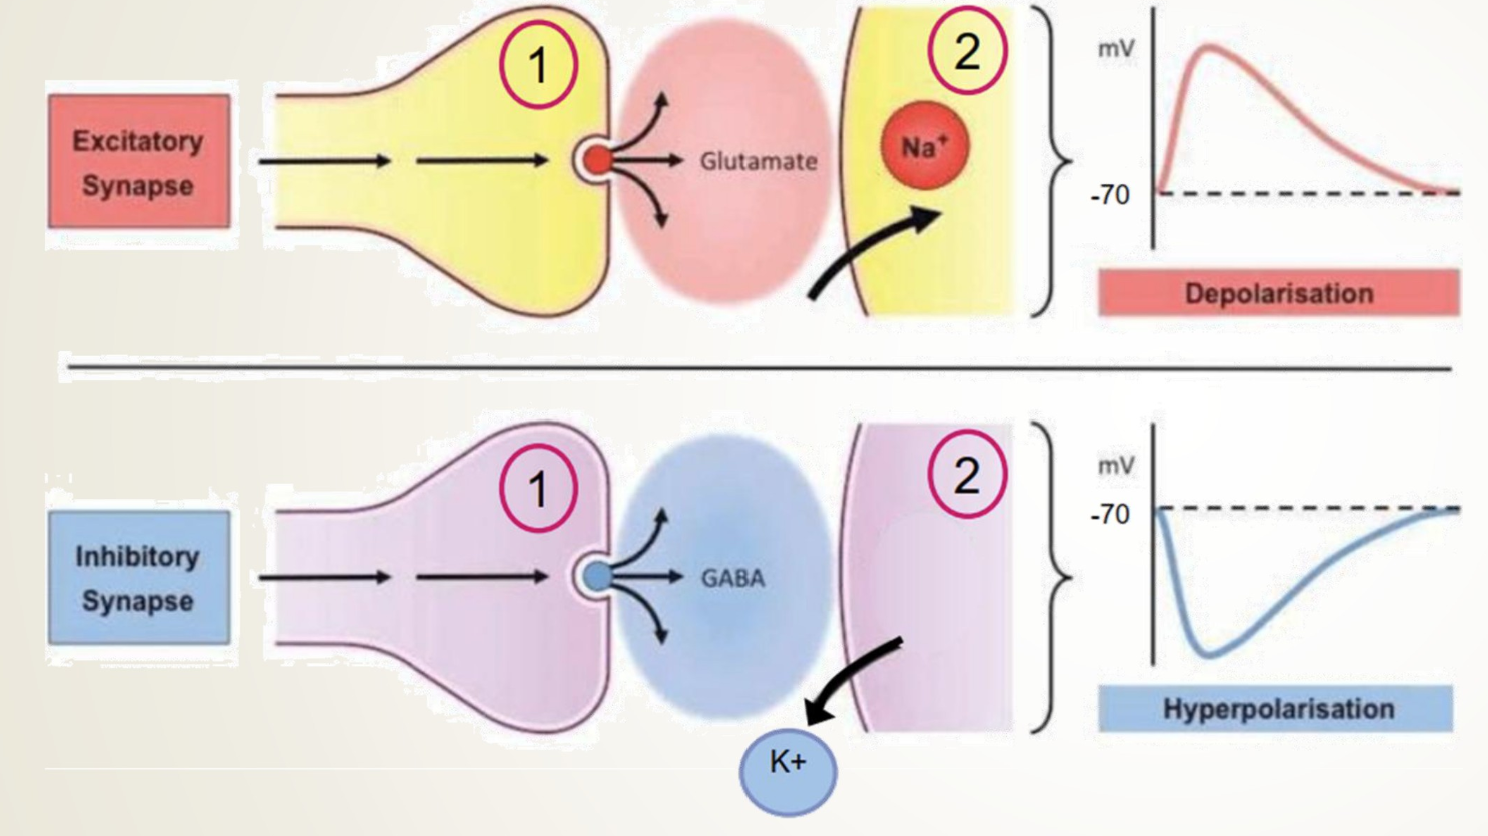
\includegraphics[width=0.7\linewidth]{immagini/eccitatoriinibitori.png}
\end{figure}
\subsection{Sommazione Spaziale e Temporale}
Il neurone trasforma gli input binari (i potenziali d'azione in arrivo) in un segnale analogico e continuo. L'integrazione dell'informazione avviene tramite due meccanismi di sommazione algebrica degli EPSP e degli IPSP:
\begin{itemize}
    \item \textbf{Sommazione Spaziale:} Più impulsi arrivano simultaneamente da neuroni presinaptici differenti su sinapsi diverse del medesimo neurone ricevente.
    \item \textbf{Sommazione Temporale:} Più impulsi arrivano in stretta e rapida sequenza sulla stessa identica sinapsi.
\end{itemize}
\begin{figure}[h]
    \centering
    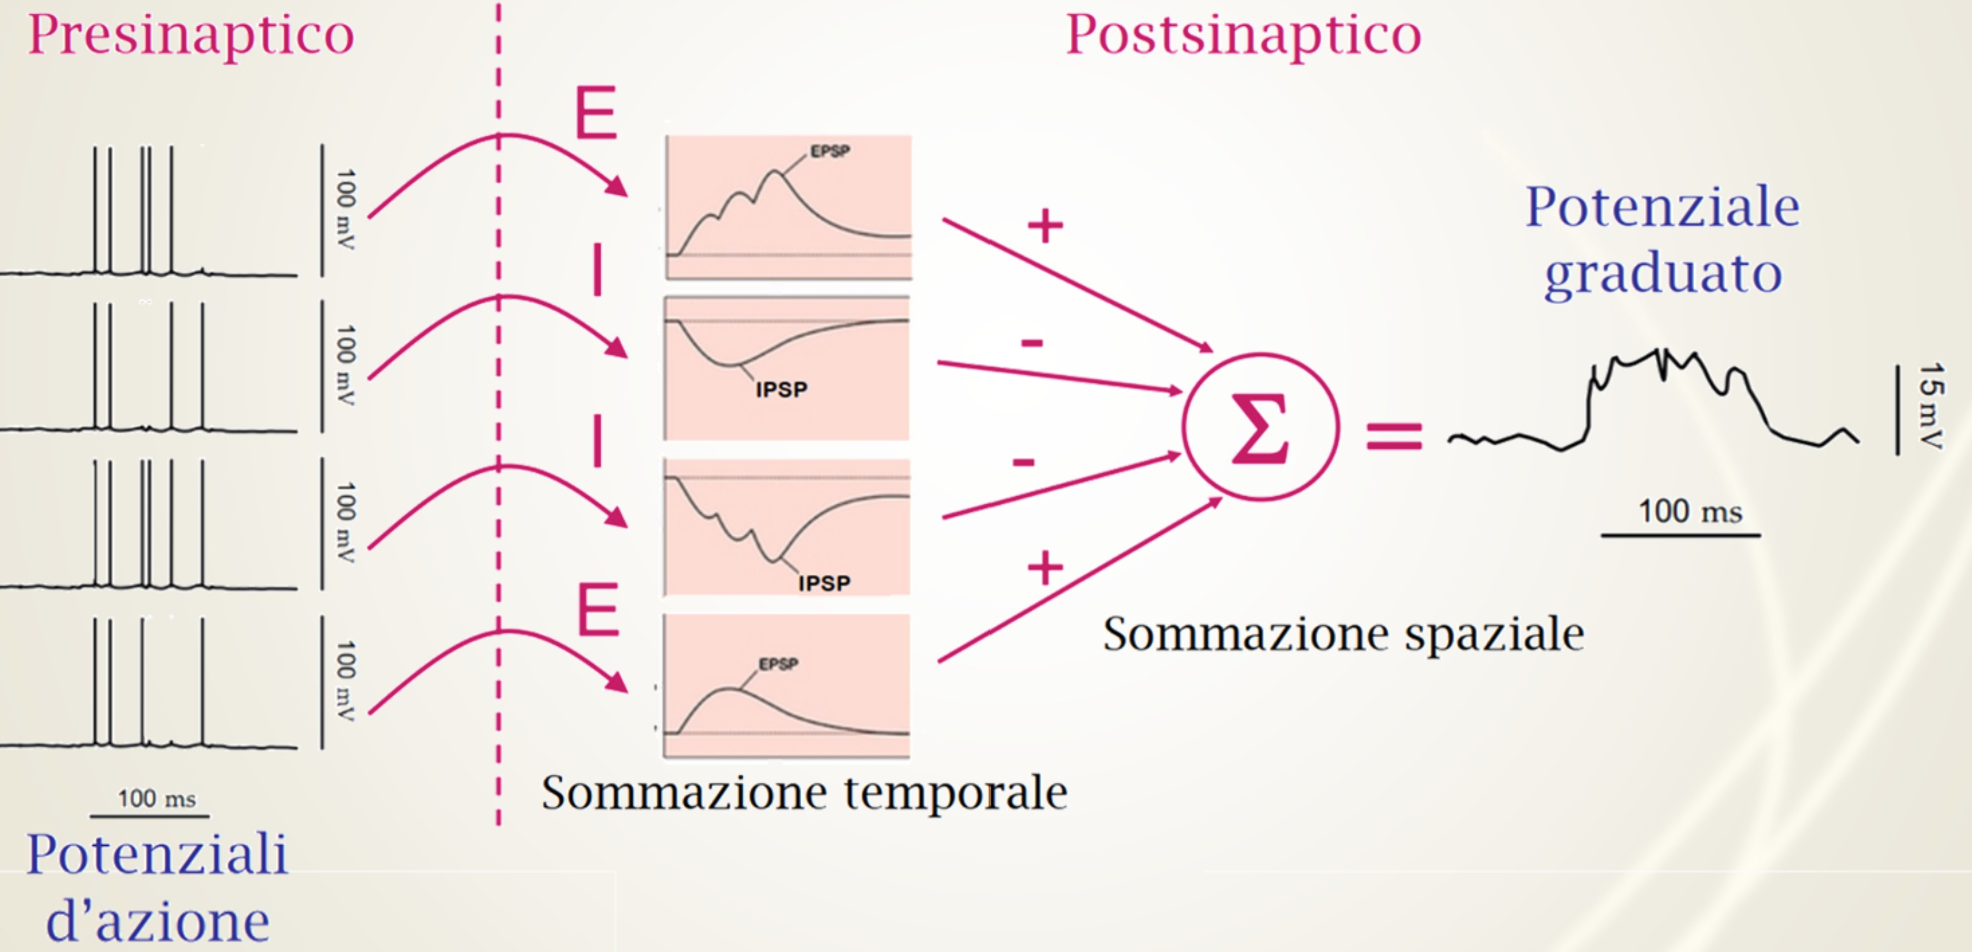
\includegraphics[width=0.7\linewidth]{immagini/integrazionepotenzialegraduato.png}
\end{figure}
Questi segnali si propagano passivamente in tutte le direzioni dalla zona di stimolazione, attenuandosi progressivamente con la distanza poiché non incontrano canali voltaggio-dipendenti lungo la membrana dendritica e somatica. Se la somma di queste perturbazioni, propagandosi fino al cono di emergenza dell'assone, raggiunge il valore di soglia, la cellula genererà un nuovo potenziale d'azione (elaborazione dell'informazione).
\begin{figure}[h]
    \centering
    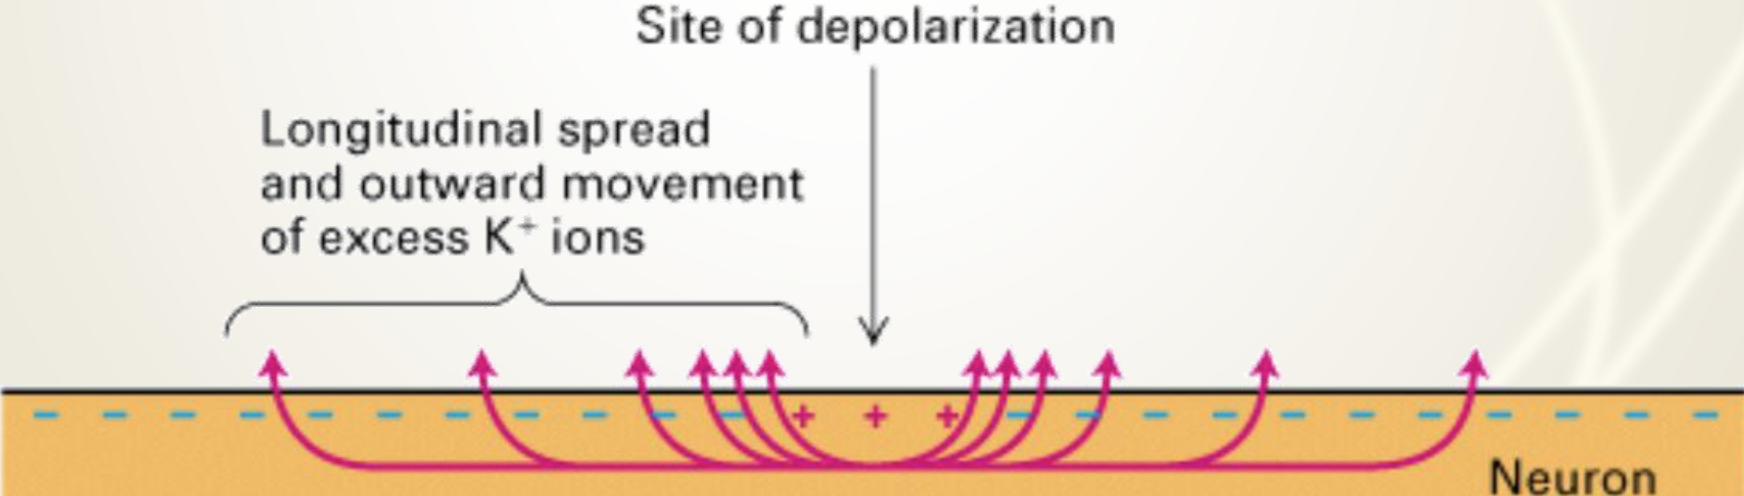
\includegraphics[width=0.75\linewidth]{immagini/propagazionepsp.png}
\end{figure}
\begin{table}[h!]
\centering
\small
\begin{tabularx}{\textwidth}{>{\raggedright\arraybackslash}X >{\raggedright\arraybackslash}X}
\toprule
\textbf{Potenziali Graduati} & \textbf{Potenziali d'Azione} \\
\midrule
Possono essere depolarizzanti o iperpolarizzanti. & Sono sempre depolarizzanti. \\\midrule
Assenza di un valore soglia. & È necessaria una depolarizzazione fino al valore soglia. \\\midrule
L'entità dipende dall'intensità dello stimolo. & Segue la legge del tutto-o-nulla; stimoli sovrasogliari producono potenziali identici. \\\midrule
Propagazione passiva che si attenua con la distanza dal sito di origine. & Propagazione attiva lungo l'assone senza alcun decremento di intensità. \\\midrule
Assenza di un periodo refrattario. & Presenza di un periodo refrattario. \\\midrule
Si verificano in gran parte delle membrane. & Si verificano solo nelle membrane eccitabili. \\\midrule
Ampiezza limitata ($\sim$ 1 mV) e durata di decine di millisecondi. & Ampiezza elevata ($\sim$ 100 mV) e durata breve ($\sim$ 1 ms). \\
\bottomrule
\end{tabularx}
\caption{Confronto tra potenziali graduati e potenziali d'azione.}
\end{table}


\section{Registrazione della risposta neuronale: registrazioni intra ed extracellulari}

Per studiare la risposta neuronale si impiegano strumenti sofisticati che permettono la registrazione extra o intracellulare, la cui scelta dipende dal tipo di potenziale da misurare e dalle condizioni sperimentali (\textit{in vivo} o \textit{in vitro}).

\subsection{Registrazioni Intracellulari}
Utilizzano microelettrodi in vetro (con un diametro in punta inferiore a 1 $\mu$m) riempiti di soluzione salina concentrata. Inseriti all'interno della cellula o a stretto contatto con essa (come nella configurazione \textit{patch}), questi elettrodi rilevano le variazioni del potenziale transmembrana interfacciandosi con un amplificatore e un oscilloscopio.
\begin{itemize}
    \item \textbf{Caratteristiche:} Sono complesse e utilizzate prevalentemente \textit{in vitro}.
    \item \textbf{Cosa misurano:} Consentono di registrare l'esatta ampiezza del potenziale di membrana in mV, riuscendo a cogliere non solo i macroscopici potenziali d'azione, ma anche i microscopici potenziali graduati (EPSP e IPSP).
    \item \textbf{Sito di registrazione:} Avvengono solitamente sul soma. Possono essere effettuate sull'assone per misurare con precisione estrema un potenziale d'azione, sebbene in questa regione non si registrino potenziali graduati.
\end{itemize}

\subsection{Registrazioni Extracellulari}
In questo caso, l'elettrodo esplorante metallico o in vetro viene posizionato nelle immediate vicinanze della membrana senza però perforarla.
\begin{itemize}
    \item \textbf{Caratteristiche:} Più semplici da eseguire, sono la scelta d'elezione per gli studi \textit{in vivo}.
    \item \textbf{Cosa misurano:} Il segnale ha un'ampiezza molto ridotta (nell'ordine di 0,1 mV) e una forma d'onda che dipende fortemente dalla geometria dell'elettrodo. Queste registrazioni non sono abbastanza sensibili da misurare i potenziali graduati; servono unicamente a rilevare il momento esatto in cui occorre un potenziale d'azione (firing rate).
\end{itemize}


\chapter{Modelli di Encoding e Decoding Neuronale}

\section{Funzione di risposta neuronale e frequenza di scarica}

Il sistema nervoso interagisce con l'ambiente esterno ricevendo stimoli sensoriali e producendo risposte motorie o cognitive. Comprendere il legame quantitativo tra le caratteristiche fisiche di uno stimolo (come l'intensità di una luce, la frequenza di un suono o la direzione di un movimento) e i potenziali d'azione generati dalle cellule nervose è l'obiettivo centrale dello studio dell'encoding e del decoding neuronale. 

L'\textbf{encoding} (o codifica) è il processo mediante il quale un neurone converte le proprietà di uno stimolo in un segnale elettrico, tipicamente rappresentato da una sequenza temporale di potenziali d'azione, detti \textit{spike}. Formalmente, l'encoding risponde alla domanda: \textit{dato uno stimolo noto, qual è la probabilità che il neurone risponda generando un determinato pattern di spike?}

Il \textbf{decoding} (o decodifica) costituisce invece il processo inverso. L'obiettivo in questo caso è dedurre lo stimolo originario a partire dall'osservazione dell'attività neuronale (il treno di spike). Questa operazione è fondamentale non solo per comprendere come il cervello interpreti i dati sensoriali, ma anche per lo sviluppo di tecnologie biomediche come le interfacce cervello-computer (Brain-Computer Interfaces). 

Trattare il \textbf{legame stimolo-risposta} in modo puramente deterministico è tuttavia impossibile. La sequenza di spike prodotta da un neurone è complessa e riflette molteplici fattori riguardanti la dinamica intrinseca della cellula: l'adattamento, lo stato dei canali ionici, il rumore interno e le fluttuazioni sinaptiche. Spesso si osservano ampie variazioni nella risposta cellulare tra una prova sperimentale (trial) e l'altra, pur mantenendo identico lo stimolo. Pertanto, sia l'encoding che il decoding devono essere affrontati con un approccio \textbf{probabilistico}, stimando la probabilità che si verifichi un certo comportamento neuronale.

\subsection{Treni di Impulsi e Frequenza di Scarica}

Ogni potenziale d'azione ha una durata molto breve e una forma d'onda stereotipata. Ai fini della codifica dell'informazione, la forma dello spike viene spesso trascurata, assimilando l'evento a un impulso puntuale. In una registrazione contenente $n$ spike, identificando con $t_i$ l'istante in cui si verifica l'i-esimo spike in un intervallo di tempo $0 \le t \le T$, l'intero treno di impulsi può essere descritto dalla \textbf{funzione di risposta neuronale} $\rho(t)$, definita tramite la somma di delta di Dirac:
\begin{equation}
\rho(t) = \sum_{i=1}^{n} \delta(t - t_i)
\end{equation}
Questa funzione non misura l'ampiezza elettrica del segnale, bensì l'occorrenza temporale esatta degli eventi.

\subsection{L'Ipotesi della Codifica in Frequenza (Rate Coding)}
L'ipotesi della codifica in frequenza suggerisce che il meccanismo primario utilizzato dal neurone per veicolare informazione sia la sua frequenza di scarica (\textit{firing rate}, indicato con $r$). Secondo questo modello classico (formalizzato già dagli studi di Adrian e Zotterman nel 1926 sulla pressione cutanea nei gatti), maggiore è l'intensità o la rilevanza dello stimolo, maggiore sarà la frequenza con cui il neurone genera potenziali d'azione.

A partire dalla funzione di risposta $\rho(t)$, esistono diverse definizioni per calcolare la frequenza di scarica:

\begin{enumerate}
    \item \textbf{Calcolo sull'intero trial}: Consiste nel contare il numero totale di spike $n$ e dividerlo per la durata del trial $T$. Matematicamente corrisponde alla media nel tempo dell'integrale della risposta:
    \begin{equation}
    r = \frac{n}{T} = \frac{1}{T} \int_{0}^{T} \rho(\tau) \, d\tau \quad \large[Hz]
    \end{equation}
    Pur fornendo una misura semplice (in Hz), questo approccio azzera completamente la risoluzione temporale, rendendo invisibili le variazioni della risposta neurale durante l'esposizione allo stimolo.
    
    \item \textbf{Calcolo locale tempo-variante ($r(t)$)}: Per preservare la dinamica della risposta, l'integrale viene valutato non più sull'intero $T$, ma all'interno di una piccola finestra temporale $\Delta t$:
    \begin{equation}
    r(t) = \frac{1}{\Delta t} \int_{t}^{t+\Delta t} \rho(\tau) \, d\tau
    \end{equation}
    Se $\Delta t$ è molto piccolo, l'affidabilità statistica sul singolo trial crolla (vi sarà al massimo 1 o 0 spike). Per ovviare a questo problema, l'esperimento viene ripetuto più volte (multi-trial) e la risposta viene mediata tra le varie prove, portando alla costruzione del PSTH (\textit{Peri-Stimulus Time Histogram}):
    \begin{equation}
    r(t) = \frac{1}{\Delta t} \int_{t}^{t+\Delta t} \langle \rho(\tau) \rangle \, d\tau
    \end{equation}
    dove il simbolo $\langle \dots \rangle$ indica la media lungo i trial. Il \textbf{PSTH} (\textit{Peri-Stimulus Time Histogram}) è un istogramma che rappresenta la frequenza media di spike (potenziali d’azione) in funzione del tempo rispetto all’inizio di uno stimolo, calcolata su più ripetizioni dello stesso esperimento (i cosiddetti trial)
\end{enumerate}

\begin{figure}[h!]
    \centering
    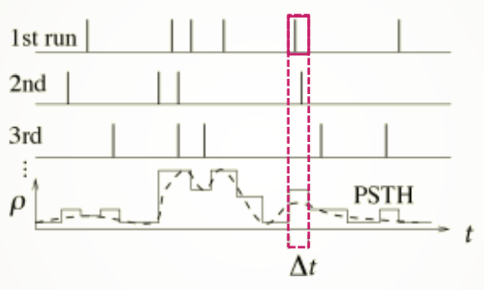
\includegraphics[width=0.5\linewidth]{immagini/multitrial.png}
\end{figure}
\newpage
Moltiplicando il firing rate istantaneo $r(t)$ per un intervallo temporale sufficientemente piccolo $\Delta t$, si ottiene il numero medio di spike attesi in quell'intervallo. Su una base di numerosi trial, $r(t)\Delta t$ esprime la probabilità che uno spike si verifichi in quell'istante:
\begin{equation}
P(\text{spike in } [t, t+\Delta t]) \approx r(t)\Delta t
\end{equation}

\subsection{Metodologie Avanzate per il Calcolo di $r(t)$}

La scelta di come calcolare $r(t)$ determina il compromesso tra risoluzione temporale e regolarità della stima (smoothness). Possiamo identificare quattro approcci principali, basati sull'utilizzo di diverse funzioni di finestratura (kernel). 

Il calcolo della frequenza istantanea può essere generalizzato come l'integrale di convoluzione tra la funzione di risposta $\rho(t)$ e una determinata funzione finestra $\omega(\tau)$ a energia unitaria:
\begin{equation}
r(t) = \int_{-\infty}^{+\infty} \omega(\tau) \rho(t-\tau) \, d\tau = \sum_{i=1}^{n} \omega(t - t_i)
\end{equation}

\begin{itemize}
    \item \textbf{1. Finestra rettangolare fissa}: Si divide l'asse temporale in bin discreti non sovrapposti. Ha il vantaggio di essere semplice da calcolare, ma offre una bassa risoluzione temporale. Assume che all'interno di ogni bin il tasso di scarica sia costante.
    \begin{figure}
        \centering
        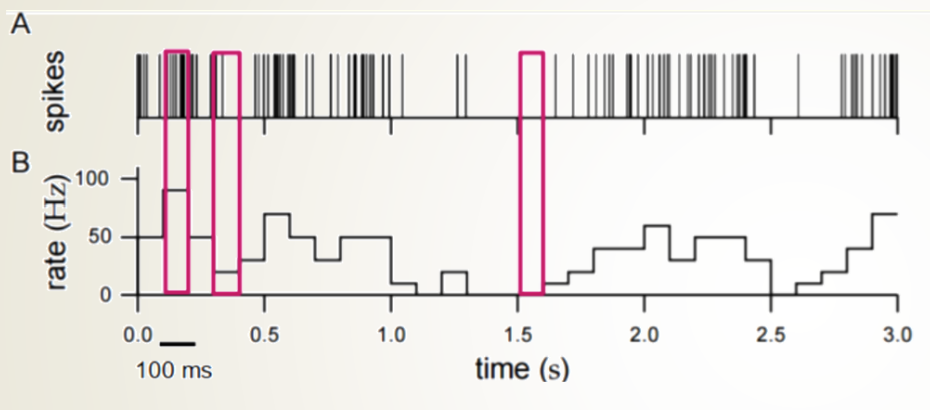
\includegraphics[width=0.5\linewidth]{immagini/rt1.png}
    \end{figure}
    \item \textbf{2. Finestra rettangolare mobile}: Un kernel rettangolare di ampiezza $\Delta t$ viene fatto scorrere in modo continuo lungo l'asse dei tempi. Questo migliora la continuità della curva di $r(t)$, ma genera misure vicine che non sono statisticamente indipendenti, poiché condividono una parte degli spike calcolati.
    \item \textbf{3. Finestra Gaussiana}: Utilizza come funzione $\omega(\tau)$ una Gaussiana a media nulla. Il parametro $\sigma_\omega$ regola l'ampiezza e quindi la risoluzione temporale:
    \begin{equation}
    \omega(\tau) = \frac{1}{\sqrt{2\pi}\sigma_\omega} e^{-\frac{\tau^2}{2\sigma_\omega^2}}
    \end{equation}
    Produce una stima estremamente fluida. Tuttavia, essendo una finestra simmetrica, "guarda" al futuro e al passato dello spike (è un filtro non causale), violando in parte il realismo fisiologico del processo di elaborazione in tempo reale da parte della sinapsi post-sinaptica.
    \item \textbf{4. Finestra Causale}: Utilizza una funzione asimmetrica ($\omega(\tau) = 0$ per $\tau < 0$). Mima più da vicino l'integrazione di membrana post-sinaptica (come la forma di un potenziale post-sinaptico eccitatorio). Sebbene sia la più accurata biologicamente, produce un segnale più asimmetrico e difficile da analizzare matematicamente rispetto alla Gaussiana.
\end{itemize}

\begin{table}[h]
\centering
\begin{tabular}{lp{4cm}p{4cm}}
\toprule
\textbf{Finestra $\omega(t)$} & \textbf{Pro} & \textbf{Contro} \\
\midrule
Rettangolare fissa & Calcolo immediato & Bassa risoluzione temporale \\
Rettangolare mobile & Migliore continuità & Misure fortemente correlate \\
Gaussiana simmetrica & $r(t)$ molto fluida e derivabile & Non causale (non realistica) \\
Filtro Causale & Rispetta la fisiologia cellulare & Matematicamente complessa \\
\bottomrule
\end{tabular}
\caption{Confronto tra le funzioni di finestratura per il calcolo di $r(t)$.}
\end{table}

%%%
\iffalse %%%%%
%%%%

\section{Le Curve di Tuning}

Una \textbf{curva di tuning} descrive l'andamento della risposta media di un neurone, espressa come $\langle r \rangle$, in funzione di una specifica caratteristica $s$ dello stimolo, considerata stazionaria durante ogni prova.

Sperimentalmente, la curva si costruisce facendo variare sistematicamente il parametro $s$ (ad esempio l'angolo visivo, il contrasto o la direzione acustica) lungo diverse ripetizioni. Per ogni valore di $s$, si calcola la frequenza di scarica media sui trial. Infine, i punti sperimentali vengono interpolati mediante una funzione matematica $f(s)$ che modella la capacità del neurone di "sintonizzarsi" su determinati parametri fisici.

Esempi classici di curve di tuning includono:
\begin{enumerate}
    \item \textbf{Neuroni della corteccia visiva primaria (orientamento)}: Rispondono in maniera selettiva a barre luminose presentate in determinati angoli. La curva di tuning assume spesso una forma Gaussiana:
    \begin{equation}
    f(s) = r_{max} e^{-\frac{1}{2}\left(\frac{s-s_{max}}{\sigma_f}\right)^2}
    \end{equation}
    dove $s_{max}$ è l'angolo preferito che evoca la scarica massima $r_{max}$, e $\sigma_f$ determina la selettività (la "larghezza" della sintonizzazione).
    
    \item \textbf{Neuroni della corteccia motoria primaria (direzione)}: La frequenza di scarica modula in base all'angolo del movimento compiuto da un arto. L'adattamento segue generalmente una legge del coseno:
    \begin{equation}
    f(s) = r_0 + (r_{max}-r_0)\cos(s-s_{max})
    \end{equation}
    dove $r_0$ fornisce un offset di frequenza a riposo.
    
    \item \textbf{Neuroni per la disparità retinica binoculare}: Implicati nella percezione della profondità spaziale, mostrano una transizione repentina (a gradino o sigmoide) in corrispondenza del passaggio dalla disparità negativa a quella positiva:
    \begin{equation}
    f(s) = \frac{r_{max}}{1+\exp[(s_{1/2}-s)/\Delta_s]}
    \end{equation}
    Questo modello indica l'esistenza di una soglia netta di attivazione rispetto alla posizione degli oggetti osservati in tre dimensioni.
\end{enumerate}

\section{Fondamenti del Decoding Neuronale e Probabilità}

Nel decodificare una risposta neuronale ci affidiamo all'uso della probabilità condizionata. L'encoding determina la probabilità $P[r \mid s]$ (la probabilità di registrare il tasso di scarica $r$ se l'ambiente presenta lo stimolo $s$). Il decoding, mediante l'inversione Bayesiana, indaga invece la $P[s \mid r]$: ricevendo un segnale di frequenza $r$, qual è lo stimolo $s$ che ha massimizzato tale probabilità?

Si consideri un classico esperimento di discriminazione visiva in cui si richiede di indicare la direzione globale di punti in movimento su uno schermo. Lo stimolo possiede due livelli di direzione (positiva +, che coincide con la preferenza del neurone, e negativa -). Un parametro cruciale è la \textbf{coerenza} del movimento: quando essa è del 100\%, tutti i punti si muovono all'unisono; allo 0\%, il moto è totalmente casuale e dominato dal rumore visivo.

Registrando il tasso di scarica $r$ del neurone a vari livelli di coerenza per entrambe le direzioni, possiamo generare due distribuzioni statistiche: $P[r \mid +]$ e $P[r \mid -]$. Assumendo che si tratti di distribuzioni gaussiane con medie distinte $\langle r \rangle_+$ e $\langle r \rangle_-$ ma varianza comune $\sigma_r^2$, possiamo definire l'indice di discriminabilità $d'$:
\begin{equation}
d' = \frac{\langle r \rangle_+ - \langle r \rangle_-}{\sigma_r}
\end{equation}
Maggiore è la coerenza dello stimolo, maggiore sarà l'allontanamento tra le due medie e, conseguentemente, l'elevato valore di $d'$, garantendo un decoding facile e accurato.

\subsection{Classificazione a Soglia}
Per operare effettivamente la discriminazione, il decoder matematico deve introdurre una soglia decisionale $z$.
Se $r \ge z$, lo stimolo è classificato come direzione (+).
Se $r < z$, lo stimolo è classificato come direzione (-).
Scegliere la corretta posizione della soglia $z$ lungo l'asse delle ascisse è un problema di ottimizzazione. Valutando le probabilità relative alla posizione di $z$, generiamo i classici indici diagnostici:
\begin{itemize}
    \item \textbf{Vero Positivo (TP)}: $\beta(z) = P[r \ge z \mid +]$ (direzione + corretta).
    \item \textbf{Falso Positivo (FP)}: $\alpha(z) = P[r \ge z \mid -]$ (direzione - confusa per +).
    \item \textbf{Vero Negativo (TN)}: $1 - \alpha(z) = P[r < z \mid -]$ (direzione - corretta).
    \item \textbf{Falso Negativo (FN)}: $1 - \beta(z) = P[r < z \mid +]$ (direzione + ignorata).
\end{itemize}

\section{Accuratezza e Curve ROC}

In ambito clinico e neuroscientifico, il compromesso tra l'identificazione corretta di eventi rari e l'evitamento dei falsi allarmi è studiato mediante la Sensibilità (\textit{True Positive Rate}, TPR) e la Specificità (\textit{True Negative Rate}, TNR). 
\begin{equation}
\text{TPR} = \frac{\text{TP}}{\text{TP} + \text{FN}}, \quad \text{TNR} = \frac{\text{TN}}{\text{TN} + \text{FP}}, \quad \text{FPR} = 1 - \text{TNR}
\end{equation}

La \textbf{curva ROC} (\textit{Receiver Operating Characteristic}) è un grafico in cui viene tracciato il TPR in funzione del FPR (cioè Sensibilità contro $1 - \text{Specificità}$) per ogni valore possibile della soglia $z$.
\begin{itemize}
    \item Se $z = 0$, tutti gli eventi cadono nella classe positiva (FPR=1, TPR=1).
    \item Se $z \to \infty$, nessun evento è classificato come positivo (FPR=0, TPR=0).
    \item Una curva coincidente con la diagonale corrisponde a un classificatore casuale (nessun guadagno predittivo, prestazioni del 50\%).
    \item Una classificazione perfetta genererebbe un punto nelle coordinate (0,1).
\end{itemize}

L'area sottesa dalla curva ROC si chiama \textbf{AUC} (\textit{Area Under Curve}). Fornisce un punteggio scalare, indipendente da una specifica soglia, che varia tra $0.5$ (caso pessimo) e $1.0$ (predizione perfetta). Statisticamente, l'AUC rappresenta la probabilità che il classificatore assegni un valore di funzione (nel nostro caso un firing rate) superiore a un'istanza positiva presa a caso rispetto a una negativa.

Applicando l'analisi ROC ai trial neurofisiologici precedentemente discussi (l'esperimento della direzione di movimento dei punti a diverse coerenze), si nota che l'AUC della risposta di un singolo neurone della corteccia visiva (misurata matematicamente) si sovrappone in maniera sorprendente alla curva psicometrica del comportamento manifesto del soggetto. In termini semplici, l'informazione codificata nella frequenza di scarica di una singola cellula è sufficiente per spiegare le decisioni motorie e percettive dell'organismo. 

\section{Conclusioni e Prospettive Cliniche}

Il modello a soglia dimostra che un decoder biologico o artificiale può sfruttare la sola frequenza statistica per interpretare il mondo in presenza di rumore. Tuttavia, si tratta di un costrutto puramente matematico e descrittivo: non considera l'architettura biologica reale delle reti cerebrali, l'integrazione di centinaia di migliaia di sinapsi o le complesse tempistiche elettrochimiche, che andrebbero investigate tramite modelli a rete più evoluti.

Ciononostante, i risultati dell'analisi del decoding hanno generato applicazioni di portata storica nella riabilitazione medica. L'acquisizione di segnali da \textit{microelectrode arrays} impiantati nel cervello permette ai computer di applicare modelli statistici e reti neurali in tempo reale. Dedurre le traiettorie motorie tridimensionali (3D arm trajectory) dal firing rate di una popolazione di cellule è il principio cardine delle \textbf{Brain-Computer Interfaces} e delle neuroprotesi. Elaborando gli spike isolati dal rumore di fondo, i decoder neuronali permettono ai pazienti con deficit motori severi di tradurre l'intento cerebrale direttamente nel controllo cinetico di bracci robotici, creando un ponte ingegneristico lì dove la biologia ha interrotto la comunicazione naturale.
\fi
\appendix
\chapter{Domande delle lezioni}
\begin{multicols}{2}
\begin{enumerate}
    \item 
\end{enumerate}
\end{multicols}

\end{document}
